\documentclass{article}

\usepackage[utf8]{inputenc}
\usepackage[T1]{fontenc}
\usepackage{lipsum}
\usepackage{graphicx}
\usepackage{amsmath}
\usepackage[margin=1in]{geometry}
\usepackage{titlesec}
\usepackage{enumitem}

\titleformat{\section} 
{\LARGE\bfseries}{\thesection}{1em}{}

\titleformat{\subsection} 
{\Large\bfseries}{\thesection}{1em}{}

\begin{document}

\pagestyle{empty}

\section*{MongoDB} 
\large

\textbf{MongoDB} fornisce un database organizzato in \textbf{collezioni}. Le collezioni contengono liste di \textbf{documenti}. Ogni documento è un insieme di \textbf{campi}.
\begin{center}
    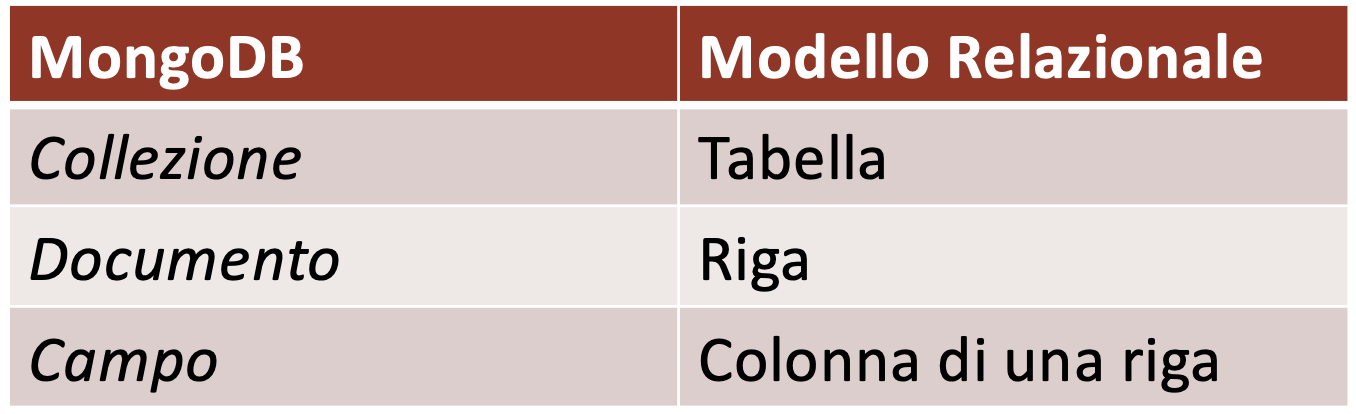
\includegraphics[width=0.5\textwidth]{foto 1.png}
\end{center}
Viene utilizzato il linguaggio \textbf{JSON} come input/output delle query di aggiornamento o selezione. Viene invece utilizzato il linguaggio \textbf{BSON}, ovvero la codifica binaria di JSON, per rappresentare i documenti internamente.\vspace{14pt}\\
Il \textit{JSON} è un \textbf{formato} per lo scambio di dati tra applicazioni. I documenti JSON sono facilmente interpretabili da macchine (\textit{machine understandability}). I dati di un documento sono racchiusi tra \{\}. I dati assuomono la forma \textbf{chiave : valore}. Alcuni esempi possono essere:
\begin{itemize}[label={ }, leftmargin=1cm]
    \itemsep0em
    \item \textbf{Numero}, intero o reale: \textbf{\{"nome": "mario", "età": 15, "punti": 13.45\}}
    \item \textbf{Stringa}, tra apici: \textbf{\{"nome": "mario", "cognome": "rossi"\}}
    \item \textbf{Booleano}, true o false: \textbf{\{"nome": "mario", "impiegato": "true"\}}
    \item \textbf{Array}, tra parentesi quadre: \textbf{\{"nome": "mario", "cap": ["134", "042"]\}}
    \item \textbf{Oggetto}, tra parentesi graffe: \textbf{\{"nome": "mario", "indirizzo": \{"città": "bologna", "via": "po", "numero": 3\}\}}\vspace{14pt}
\end{itemize}
Per avviare il \textbf{server} e la \textbf{shell} di MongoDB vengono utilizzati i seguenti comandi:
\begin{itemize}[label={ }, leftmargin=1cm]
    \itemsep0em
    \item \textit{mongodb}\quad (demone in ascolto sulla porta)
    \item \textit{mongo}\quad (shell client)
\end{itemize}
Per la \textbf{creazione} di un database o per \textbf{utilizzarlo} viene utilizzato il seguente comando:
\begin{itemize}[label={ }, leftmargin=1cm]
    \itemsep0em
    \item \textit{use provaDB}
\end{itemize}
Per la creazione di una \textbf{collezione}, anche vuota, viene utilizzato il seguente comando:
\begin{itemize}[label={ }, leftmargin=1cm]
    \itemsep0em
    \item \textit{db.createCollection("circoli");}
\end{itemize}
Alcuni comandi della shell di MongoDB sono:
\begin{center}
    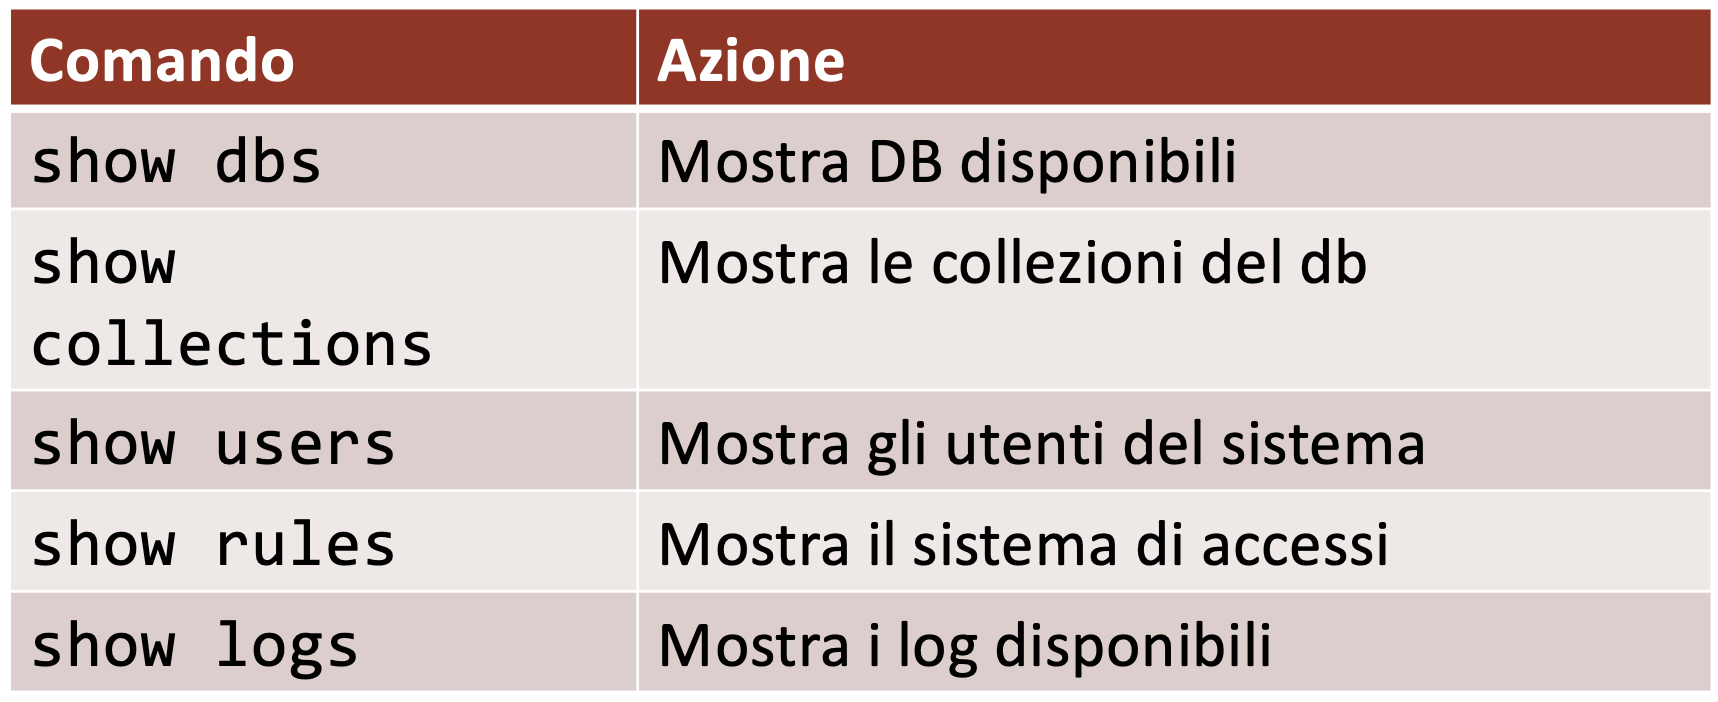
\includegraphics[width=0.7\textwidth]{foto 2.png}
\end{center}
Un \textbf{documento} in MongoDB segue il concetto dell'oggetto \textbf{JSON}.\\
Nella stessa collezione è possibile inserire documenti \textbf{eterogenei}, ossia con \textbf{struttue campo/valore} differenti.
\begin{center}
    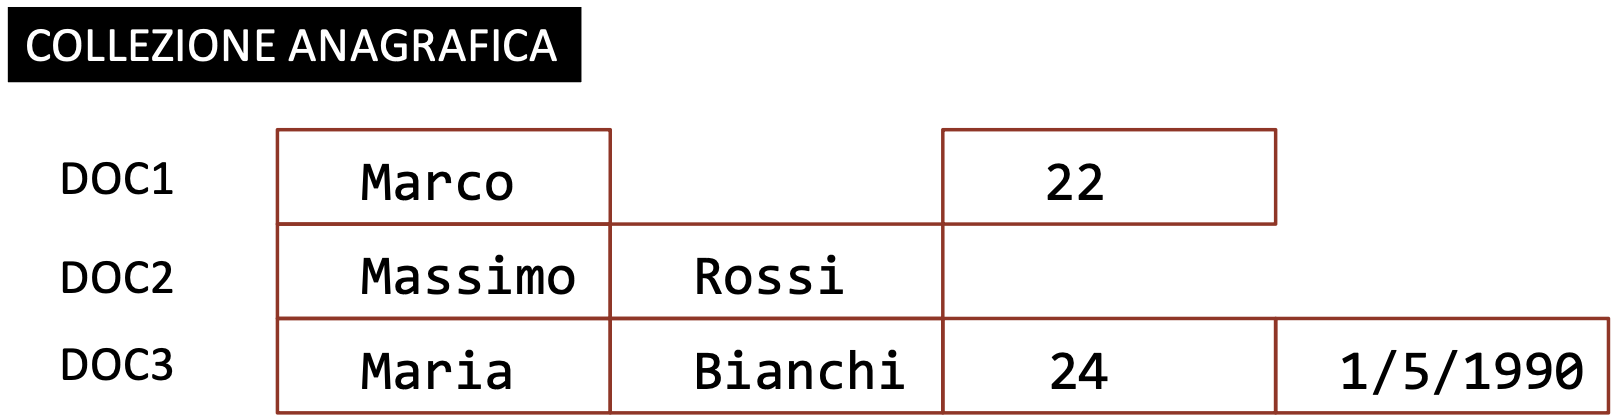
\includegraphics[width=0.6\textwidth]{foto 3.png}
\end{center}
Non è possibile rappresentare casistiche simili nel modello relazionale, a meno di usare valori NULL. Un'altra differenza tra il modello relazionale ed il modello non relazionale è la possibilità di poter inserire tipi complessi nei modelli non relazionali. Negli RDBMS invece, seguendo la \textit{prima forma normale}, è possibile avere soltanto tipi semplici all'interno di una colonna.\vspace{14pt}\\
\textit{\textbf{Inserimento} di un documento in una collezione}
\begin{itemize}[label={ }, leftmargin=1cm]
    \itemsep0em
    \item \textit{db.NOMECOLLEZIONE.insert(DOCUMENTO)}
\end{itemize}
Ogni documento contiene un campo \textit{\textunderscore id} che corrisponde alla \textbf{chiave primaria} della collezione. Il campo \textunderscore id può essere definito \textbf{esplicitamente}, o viene aggiunto in maniera implicita da MongoDB.\vspace{14pt}\\
\textit{\textbf{Rimozione} di un documento in una collezione}
\begin{itemize}[label={ }, leftmargin=1cm]
    \itemsep0em
    \item \textit{db.NOMECOLLEZIONE.remove(\{\})}\quad svuota la collezione
    \item \textit{db.anagrafica.remove(\{\})}\quad DELETE FROM anagrafica
    \item \textit{db.NOMECOLLEZIONE.remove(SELETTORE)}\quad eliminando dalla collezione tutti i documenti che fanno matching con il selettore
\end{itemize}
Il \textbf{selettore} è un documento JSON, formattato ad esempio come segue:
\begin{center}
    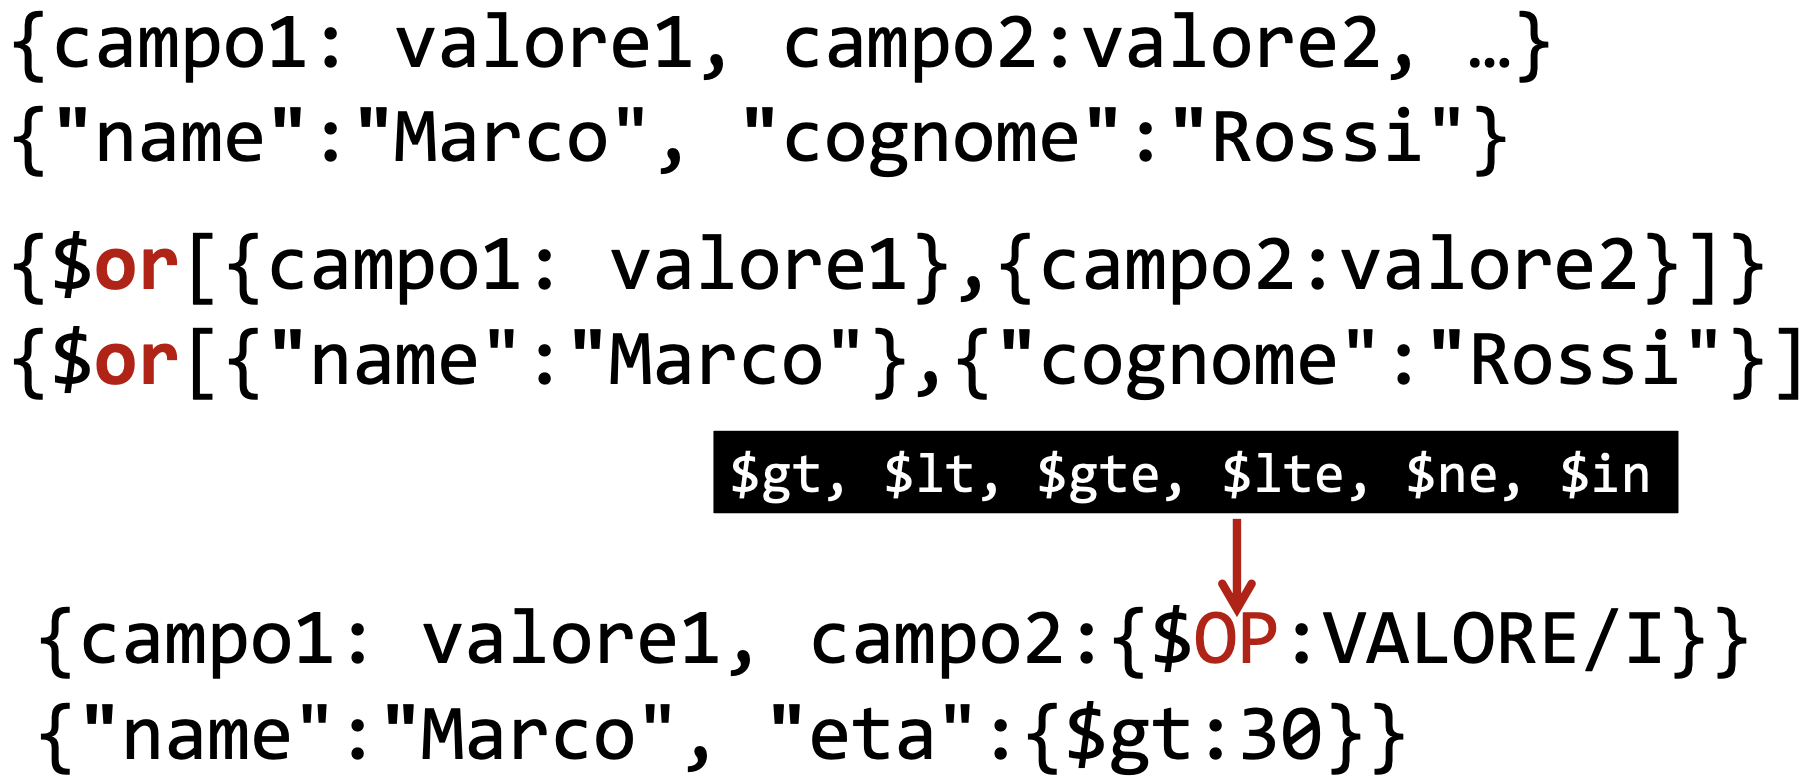
\includegraphics[width=0.7\textwidth]{foto 4.png}\vspace{14pt}\\
\end{center}
\textit{\textbf{Aggiornamento} di un documento in una collezione}
\begin{itemize}[label={ }, leftmargin=1cm]
    \itemsep0em
    \item \textit{db.NOMECOLLEZIONE.update(SELETTORE, CAMPI))}
    \item \textit{db.NOMECOLLEZIONE.update(SELETTORE, \{\$SET: CAMPI\}))}
    \item \textit{db.NOMECOLLEZIONE.update(SELETTORE, \{\$PUSH: CAMPI\}))}
    \item \textit{db.anagrafica.update(\{"name": "Mario"\},\{"eta": 45\})}\quad sostituisce il documento relativo all'impiegato Mario
    \item \textit{db.anagrafica.update(\{"name": "Mario"\},\{\$set:\{"eta": 45\}\})}\quad nel documento relativo all'impiegato Mario, aggiorna il campo età ponendolo a 45
    \item \textit{db.anagrafica.update(\{"name": "Mario"\},\{\$set:\{"eta": 45\},\{multi:true\}\})}\quad in tutti i documenti relativi all'impiegato Mario, si aggiorna il campo età ponendolo pari a 45
    \item \textit{db.anagrafica.update(\{"name": "Mario"\},\{\$push:\{"eta": 45\}\})}\quad nel documento relativo all'impiegato Mario, si aggiunge un nuovo campo età(array), settandolo a 45\\
\end{itemize}
\textit{\textbf{Ricerca} di un documento all'interno in una collezione}
\begin{itemize}[label={ }, leftmargin=1cm]
    \itemsep0em
    \item \textit{db.NOMECOLLEZIONE.find()}\quad restituisce tutt i documenti presenti nella collezione
    \item \textit{db.NOMECOLLEZIONE.find(SELETTORE)}\quad restituisce tutt i documenti i cui campi rispettino la condizione espressa nella query
    \item \textit{db.NOMECOLLEZIONE.find(SELETTORE, PROJECTION)}\quad restituisce tutt i campi projection dei documenti, i cui campi rispettino la condizione espressa nella query
\end{itemize}
Alcuni esempi di utilizzo del costrutto di find possono essere:
\begin{itemize}[label={ }, leftmargin=1cm]
    \itemsep0em
    \item \textit{db.anagrafica.find()}\quad SELECT * FROM anagrafica
    \item \textit{db.anagrafica.find(\{"nome": "Mario", "eta": 30\})}\quad SELECT * FROM anagrafica WHERE ((Nome = "Mario") AND (ETA = 30))
    \item \textit{db.anagrafica.find(\{"nome": "Mario"\}, \{"eta": 1\})}\quad SELECT \textunderscore ID, ETA FROM anagrafica WHERE (Nome = "Mario")
    \item \textit{db.anagrafica.find(\{\$or:[\{"nome": "Mario"\},\{"eta": 56\}]\},\{"eta": 1\})}\quad SELECT \textunderscore ID, ETA FROM anagrafica WHERE ((Nome = "Mario") OR (ETA = 56))
    \item \textit{db.anagrafica.find(\{"eta": \{\$gte: 60\}\})}\quad SELECT * FROM anagrafica WHERE (ETA >= 60)
\end{itemize}
\textit{Operatori di ordinamento, conteggio e filtro duplicati}\\
Per l'\textbf{ordinamento di una collezione} viene usato il seguente comando:
\begin{itemize}[label={ }, leftmargin=1cm]
    \itemsep0em
    \item \textit{db.NOMECOLLEZIONE.find(\dots).sort(CAMPO/CAMPI)}
    \item \textit{db.anagrafica.find(\{"name": "Mario"\}).sort("eta": 1)}
    \item 1 ordinamento crescente, -1 ordinamento decrescente
\end{itemize}
Per \textbf{contare i documenti} viene usato il seguente comando:
\begin{itemize}[label={ }, leftmargin=1cm]
    \itemsep0em
    \item \textit{db.NOMECOLLEZIONE.find(\dots).count()}
\end{itemize}
Per \textbf{filtrare i documenti duplicati} viene usato il seguente comando:
\begin{itemize}[label={ }, leftmargin=1cm]
    \itemsep0em
    \item \textit{db.NOMECOLLEZIONE.distinct([CAMPO], SELETTORE)}
    \item \textit{db.anagrafica.distinct(\{"eta": 1\},\{"name": "Mario"\})}\vspace{14pt}\\
\end{itemize}
\textit{Estensione procedurale di MongoDB}\\
Il file di script può contenere \textbf{costrutti iterativi e/o di selezione}:
\begin{itemize}[label={ }, leftmargin=1cm]
    \itemsep0em
    \item \textit{while(condizione) \{ LISTA COMANDI \}}
    \item \textit{if(condizione) \{ LISTA COMANDI \}}
    \item \textit{else(condizione) \{ LISTA COMANDI \}}
\end{itemize}
I \textbf{cursori} vengono usati per scorrere il risultato di una query:
\begin{itemize}[label={ }, leftmargin=1cm]
    \itemsep0em
    \item \textit{cursor = db.collection.find(\dots);}
    \item \textit{while(cursor.hasNext() )\{}
    \item \quad \textit{printjson(cursor.next() );}
    \item \textit{\}}\\
\end{itemize}
Supponiamo di dover rappresentare \textbf{correlazioni tra collezioni} in MongoDB. Come tutti i sistemi NoSQL, MongoDB non mette a disposizione i costrutti di vincoli di integrità referenziale tra collezioni/tabelle.\\
Le \textbf{correlazioni} possono essere costruite esplicitamente mediante \textbf{campi} \textit{replicati} tra più collezioni.
\begin{itemize}[label={ }, leftmargin=1cm]
    \itemsep0em
    \item \textit{db.circoli.insert(\{"nome": "tennis2000", "citta": "Bologna"\})}
    \item \textit{db.soci.insert(\{"nome": "Mario", "cognome": "Rossi", "nomeCircolo": "tennis2000"\})}
\end{itemize}
Le associazioni \textit{uno a molti}, o \textit{molti a molti}, tra documenti di diverse collezioni possono essere rappresentate sfruttando il fatto che in MongoDB il valore di un campo può essere anche un \textbf{array}, o una struttura complessa come un documento annidato.
\begin{itemize}[label={ }, leftmargin=1cm]
    \itemsep0em
    \item \textit{db.soci.insert(\{"name": "Mario", "cognome": "Rossi", "circolo": \{\dots\}\})}
\end{itemize}
Si presenta un problema: come scrivere la query che restituisce nome e cognome dei soci che partecipano a circoli situati a Bologna, implementando il \textbf{JOIN tra collezioni}?\\
Una prima soluzione è quella di usare l'operatore di \textbf{lookup}.\\
Una seconda soluzione è quella di usare \textbf{due query}:
\begin{itemize}[label={ }, leftmargin=1cm]
    \itemsep0em
    \item \textit{db.circoli.find(\{"luogo": "Bologna",\{\}\})}\quad output:\{"\textunderscore id": "432"\}
    \item \textit{db.soci.find(\{"circolo": "432"\}, \{"nome": 1, "cognome": 1\})}\\
\end{itemize}
\textit{Aggregazione dati mediante operatore di \textbf{aggregate}}\\
Consente di implementare una \textbf{pipeline} di operazioni da eseguire sulla base di dati. Ad ogni passo della pipeline, vengono eseguite operazioni che prendono in input dei documenti JSON e producono in output documenti JSON.
\begin{center}
    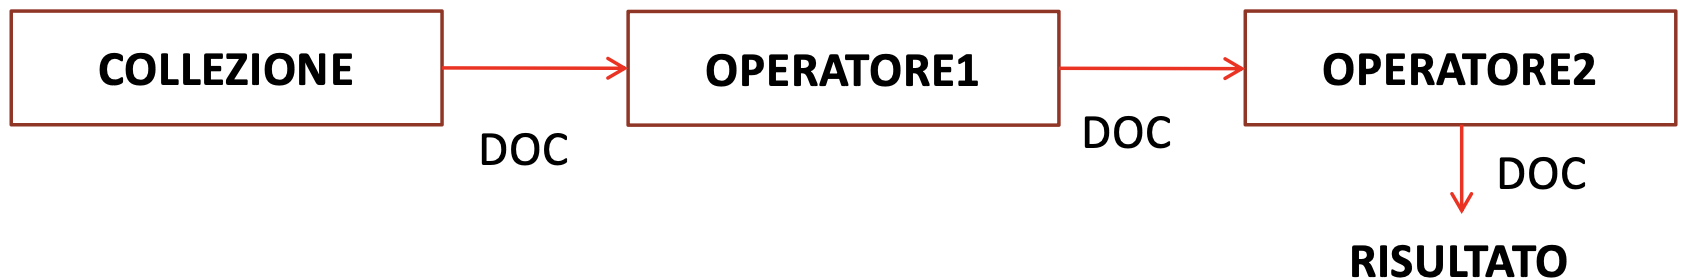
\includegraphics[width=0.7\textwidth]{foto 5.png}\vspace{14pt}\\
\end{center}
Alcuni esempi di operatori sono:
\begin{itemize}[label={-}, leftmargin=1cm]
    \itemsep0em
    \item \textbf{\$geonear}: ordina i documenti dal più lontano al più vicino rispetto ad una posizione data
    \item \textbf{\$match}: seleziona solo alcuni documenti che soddisfano le condizioni fornite in input
    \item \textbf{\$project}: seleziona i campi prescelti
    \item \textbf{\$group}: raggruppa in base ad uno o più campi
    \item \textbf{\$limit}: seleziona i primi n documenti del JSON
    \item \textbf{\$sort}: ordina il JSON in base ad alcuni campi
    \item \textbf{\$out}: scrive l'output su una collezione
    \item \textbf{\$lookup}: consente di effettuare il \textbf{join} tra collezioni che appartengono allo stesso database\\
\end{itemize}
Un esempio di sintassi del \textit{lookup} può essere:
\begin{itemize}[label={ }, leftmargin=1cm]
    \itemsep0em
    \item \textit{\{\$lookup: \{}
    \item \quad \textit{from: collezione su cui fare il join,}
    \item \quad \textit{localField: campo della collezione di partenza,}
    \item \quad \textit{foreignField: campo della collezione del from,}
    \item \quad \textit{as: nome del campo destinazione}
    \item \quad \textit{\}}
    \item \textit{\}}
\end{itemize}
Un esempio di aggregazione dati mediante l'operatore di \textit{aggregate} potrebbe essere:
\begin{itemize}[label={ }, leftmargin=1cm]
    \itemsep0em
    \item \textit{db.NOMECOLLEZIONE.aggregate([OPERATORE1, OPERATORE2,\dots , OPERATOREN])}
    \item \textit{db.anagrafica.aggregate([
    \item \quad \{\$match: \{"name": "A"\}\},
    \item \quad \{\$group: \{\textunderscore id: "\$customId", total: \{\$sum: "\$amount"\}\}\},
    \item \quad ])}
\end{itemize}

\subsection*{Sharding}
\large

Lo \textbf{sharding} è un processo di \textit{suddivisione dei dati} su un cluster di server MongoDB. La distribuzione dei dati viene effettuata per avere una maggiore capacità di storage e computazionale, una ridondanza dei dati e la disponibilità del servizio continua.\\
Per effettuare la suddivisione dei dati in un sistema distribuito è necessario definire una \textbf{shard key}. La chiave \textbf{deve essere presente su tutti i documenti di una collezione}. In base al valore della chiave, si suddivide la collezione in \textbf{segmenti}, o \textbf{chunks}.\\
Gruppi diversi di chunk vengono assegnati ai diversi nodi del cluster. Si pone quindi la problematica dell'\textbf{allocazione}. Si osservino due soluzioni distinte:
\begin{itemize}[label={-}, leftmargin=1cm]
    \itemsep0em
    \item \textbf{Range-Based Sharding}: individua il valore massimo e minimo della chiave. Ogni chunk corrisponde ad un intervallo [K - i, K + i]
    \item \textbf{Hash-Based Sharding}: MongoDB applica la funzione \textbf{hash(\#chunk)}. Il risultato della funzione determina il server
\end{itemize}
Se fosse necessario svolgere delle ottimizzazioni a run-time, sono presenti due metodologie principali:
\begin{itemize}[label={-}, leftmargin=1cm]
    \itemsep0em
    \item \textbf{Splitting}: se un chunk cresce troppo in dimensione, esso viene splittato in più parti. L'operazione viene eseguita su un server, e non comprende la migrazione del chunk stesso
    \begin{center}
        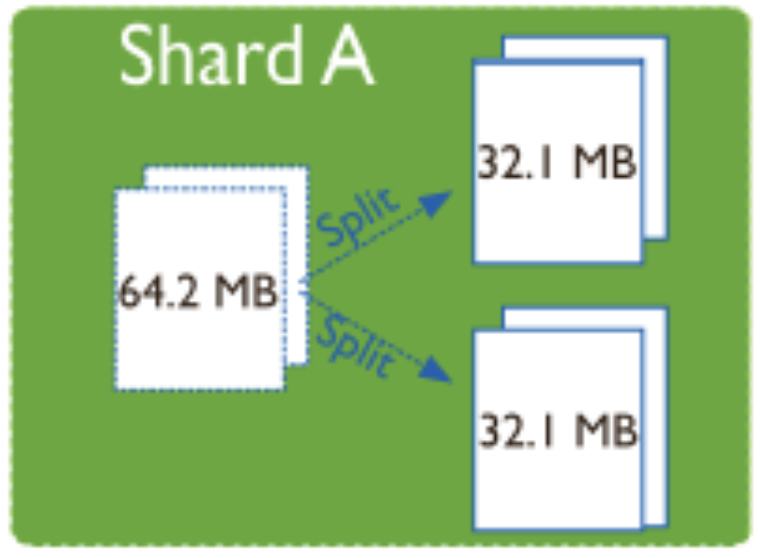
\includegraphics[width=0.2\textwidth]{foto 6.png}
    \end{center}
    \item \textbf{Balancing}: il \textbf{balancer} viene eseguito in \textbf{background} e tiene traccia del numero di chunk gestito da ciascun server. In caso di allocazione non bilanciata, il \textit{balancer} provvede a \textbf{migrare i chunk} tra server differenti, dal più carico al più scarico
    \begin{center}
        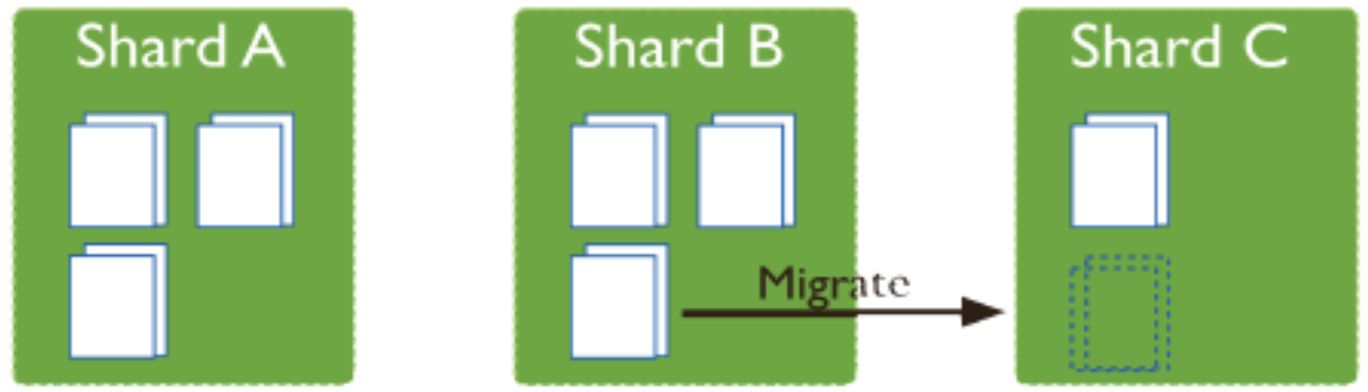
\includegraphics[width=0.5\textwidth]{foto 7.png}
    \end{center}
\end{itemize}
\end{document}